% ---------------------------------------------------
% ----- Introduction of the template
% ----- for Bachelor-, Master thesis and class papers
% ---------------------------------------------------
%  Created by C. Müller-Birn on 2012-08-17, CC-BY-SA 3.0.
%  Last upadte: C. Müller-Birn 2015-11-27 
%  Freie Universität Berlin, Institute of Computer Science, Human Centered Computing. 
%
\chapter{Einleitung}
\label{chap:introduction}

Im folgenden werden Ihnen Hinweise zur Strukturierung und zum Inhalt des ersten Kapitels gegeben.

\section{Thema und Kontext}
\begin{itemize}
	\item Wo setze ich an? (Problemstellung / Ausgangslage)      
	\item Identifikation der signifikanten Problemen im betrachteten Forschungsbereich  
	\item Ein kurzer Überblick über den aktuellen Forschungsstand in dem Bereich inklusive vorhandener Lösungen (ausführlicher dann in den Folgeabschnitten)
\end{itemize}

\section{Zielsetzung der Arbeit}
\begin{itemize}
	\item Was sind die mit dieser Arbeit verfolgten Ziele? Welches Problem soll gelöst werden?
	\item Eine Beschreibung der ersten Ideen, der vorgeschlagene Ansatz und die aktuell erreichten Resultate 
	\item Eine Beschreibung, welchen Beitrag die Arbeit leistet, um das vorgestellte Problem zu lösen
	\item Eine Diskussion, wie die vorgeschlagene Lösung sich von bestehenden unterscheidet, was ist neu oder besser?
\end{itemize}

\section{Vorgehen bei der Umsetzung}
\begin{itemize}
	\item Wie will ich meine Ziele erreichen? (Methodische Überlegungen)
	\item Darstellung zum Forschungsdesign.
	\item Insbesondere bei Master: Wie kann die Zielerreichung ``gemessen'' werden? 
\end{itemize}  	

\section{Aufbau der Arbeit}
\begin{itemize}
	\item Welche Schritte werden durchlaufen, um die Ziele zu erreichen?
	\item An dieser Stelle ist beispielsweise eine Grafik hilfreich, um den Aufbau der Arbeit und welche Ergebnisse/Erkenntnisse wo genutzt werden, zu visualisieren. 
	\item Ebenfalls sollten noch Anmerkungen zur Gestaltung der Arbeit gegeben werden, vor allem, da in vielen deutschen Arbeiten englische Fachbegriffe verwendet werden. Ein solcher Text könnte folgendermaßen lauten: 
		\begin{itemize}
			\item ``Abschließend sind hier noch eine Anmerkungen zur Gestaltung der vorliegenden Arbeit. Für die im Folgenden verwendeten personenbezogene Ausdrücke wurde, um die Lesbarkeit der Arbeit zu erhöhen, die männliche Schreibweise gewählt. Des Weiteren werden eine Reihe von englischen Bezeichnungen verwendet, um einerseits dem interessierten Leser das Studium der häufig vorliegenden englischen Originalliteratur zu erleichtern oder andererseits bestehende Fachbegriffe nicht durch die Übersetzung zu verfälschen. Diese Begriffe sind vom herkömmlichen Text in kursiver Schrift unterschieden.''
		\end{itemize}
\end{itemize}

\begin{figure}[!ht]
	% Mit [!h] wird die Position der Grafik bestimmt. So bedeutet h=here und mit dem "!" (Ausrufezeichen) wird dieser Befehl verstärkt. Weitere Möglichkeiten sind : t=top und b=bottom. Zumeist wird angegeben, in welcher Reihenfolge LaTeX versuchen soll das Bild einzufügen, z.B. [!htb].
	\centering
		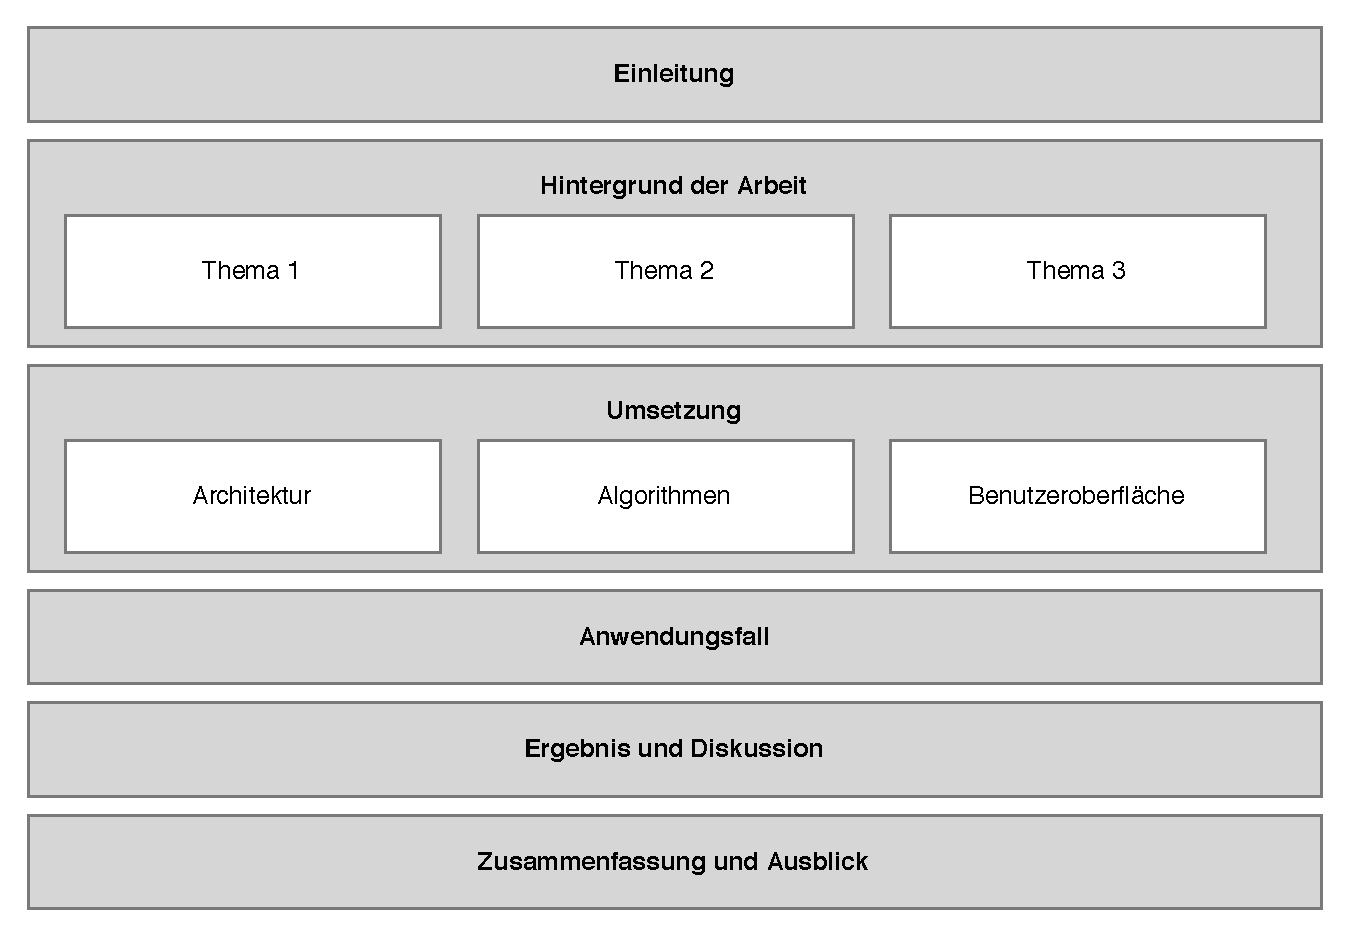
\includegraphics[width=0.95\textwidth]{pics/structure.pdf}
	\caption[Beispiel einer möglichen Darstellung zum Aufbau der Arbeit]{Beispiel einer möglichen Darstellung zum Aufbau der Arbeit (vgl. Beschreibung Abschnitt  \ref{chap:chapters}).} 
	% Mit Hilfe von caption wird die Bildunterschrift erzeugt. Der Text in geschweiften Klammern erscheint im Text, während der Text in eckigen Klammern sich dann empfiehlt, wenn die Beschreibung besonders lang ist, denn diese wird dann im Bildverzeichnis verwendet. Diese Kurzbeschreibung kann auch weggelassen werden. 
	\label{fig:structurethesis}
\end{figure}